\documentclass[12pt,a4paper]{article}
%packages
\usepackage[utf8]{inputenc}
\usepackage[T1]{fontenc}
\usepackage[english]{babel}
\usepackage{amsmath}
\usepackage{amsfonts}
\usepackage{amssymb}
\usepackage{graphicx}
\usepackage{hyperref}
\usepackage{tikz}
\usetikzlibrary{positioning,angles,quotes}
\usepackage[acronym]{glossaries}
%glossary 
\newacronym{qrl}{QRL}{Quantum Reinforcement Learning}
\newacronym{ai}{AI}{Artificial Intelligence}
\newacronym{drl}{DRL}{Deep Reinforcement Learning}
\newacronym{rl}{RL}{Reinforcement Learning}
\newacronym{qc}{QC}{Quantum Computing}
\newacronym{nn}{NN}{Neural Networks}
\newacronym{mdp}{MDP}{Markov Decision Process}
\newacronym{vqa}{VQA}{Variational Quantum Algorithm}
\makenoidxglossaries
%settings
\usepackage[left=2.00cm, right=2.00cm, top=2.00cm, bottom=2.00cm]{geometry}
\author{Matteo Conterno}
\title{Prospects of quantum computing approach to reinforcement learning}
%start of document
\begin{document}
	\maketitle
	\begin{center}
	\section*{Abstract}
\end{center}
Reinforcement learning is one of three major techniques that allows a model to learn, especially this technique focus on how to create an optimal agent able to reach an objective by interacting with an environment. 
This thesis tries to analyze the possible potentials and advantages that would derive by using quantum circuits with neural networks; 
analyzing and explaining how it is possible to create hybrid algorithms that exploit the advantages of both the classical and quantum algorithm, expanding the applicability not only on simulators, but even on quantum devices such as Rigetti and IonQ's processors through the amazon AWS braket service. 
Lastly it is analyzed how the quantum noise influence an optimal model obtained through a simulator, by testing it on a quantum processor to understand if it is possible to use the hybrid algorithm on the actual devices.
\newline
\begin{center}
	\printglossary
\end{center}

	{
	 	\hypersetup{hidelinks}
		\tableofcontents
	}
	
	\section{Introduction to Deep Reinforcement Learning and Quantum Computing}
%introduction
This section of the thesis is created so that it can give an introduction to the fields of \acrlong{ai}(\acrshort{ai}) specifically to \acrlong{drl}(\acrshort{drl}) and the basis of \acrlong{qc}(\acrshort{qc}) in order to understand afterward the fusion of these two different fields on \acrlong{qrl}(\acrshort{qrl}). If already expert on these subjects fell free to skip at the next section.
%subsection of learnings
\subsection{Approaches of learning}
Currently any kind of \acrshort{ai} requires the following components to learn:
\begin{itemize}
	\item Data
	\item Model
	\item Approach of learning
\end{itemize}
Data is necessary in every \acrshort{ai} model, the amount and quality can heavily influence the ability to correctly and efficiently reach his goal. 
The model is an algorithm that, given some data and a predefined objective, tries to complete his task using some learning approach. In order to check if the model has correctly learned, it will be later tested on unseen data and evaluated to understand if it is able to replicate the performances given a similar dataset.\\
The approach of learning specify how the model can learn to complete his task. At the moment there are three major ways:
\begin{itemize}
	\item \textbf{Supervised learning} : the data is already labeled, this means that we can define when the model is incorrect or correct.
	\item \textbf{Unspervised learning} : the data is not labeled, this means that we can't define easily when the model is correct or incorrect and the model must uncover some pattern.
	\item \textbf{Reinforcement learning} : an agent interact with the environment in order to become the most optimal agent to complete the task.
\end{itemize}
This thesis will focalize mainly on the reinforcement learning approach and especially on the \acrfull{drl} which uses \acrfull{nn} to define the most optimal agent.
In this thesis the focus is on what kind of advantage can be obtained by using a quantum algorithm such as \acrfull{vqa}, this technique can be even used in other context and applications. Futhermore it has been demostrated that \acrshort{vqa} and \acrshort{nn} share some similarities and properties. The main drawback is the fact that when a \acrshort{vqa} is trained on a classical device, there is a major overhead of time due to simulation of the quantum circuit implemented and the number of qubits is limited.
%sub section of reinforcement learning
\subsection{Reinforcement Learning}
As said earlier a reinforcement learning approach consist of creating the most optimal agent able to complete a predefined task by interacting with the environment and taking some action. Questions arises about: how can be defined if an action is good or bad? How to model a dynamic environment? The answer is given by using a statistical model called \acrfull{mdp} .
\subsubsection{Markov Decision Process}
In order to model a dynamic environment where an action can influence the sistem it is necessary to use the \acrfull{mdp} which is an extension of Markov chains; these are a stochastic model that is able to describe a sequence of possible events that satisfy the Markov propriety, that is each event depends only on the previous event.\\
It is necessary to note that an \acrshort{mdp} is based on Markov Chains that not only model the states, but even the time and this can be defined as continuous or discretized.
\acrshort{mdp} is an extension of Markov Chains because the agent can influence the state of environment and outcome, so a framework is necessary to define even his decisions and their consequences. An \acrshort{mdp} is defined as a 4-tuple containing the following elements:
\begin{itemize}
	\item $S$ : set of states
	\item $A$ : set of actions
	\item $P_a (s, s') = Pr(s_{t+1} = s' \vert s_{t} = s)$ : is the transition probability of going from state $s$ to $s'$ by taking an action $a$
	\item $R_{a}(s,s')$ is the immediate reward obtained by transitioning from state $s$ to $s'$ by action $a$
\end{itemize}
The difference with a Markov chains is the presence of $P_a (s, s')$ and $R_{a}(s,s')$ which are necessary for the decision process, to see an example graph of and MDP see Figure \ref{fig:mdpgraph}.
\begin{figure}[!ht]
	\centering
	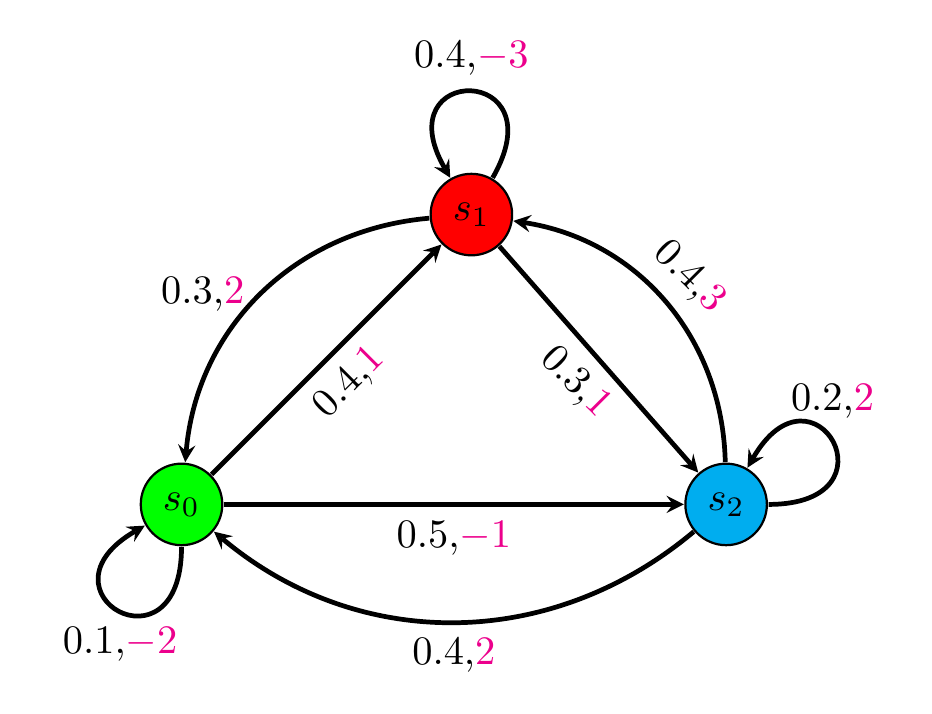
\begin{tikzpicture}[thick,scale=1.46, every node/.style={transform shape}, line width=0.6mm]
		\tikzstyle{round}=[thick,draw=black,circle]
		\node[round, fill=green] (s0) {$s_0$};
		\node[round,above right=20mm and 20mm of s0, fill=red] (s1) {$s_1$};
		\node[round, right=40mm of s0, fill=cyan] (s2) {$s_2$};
		\draw[-stealth] (s0) -- node[below, rotate=45]
		{\color{black} $0.4$\color{black},\color{magenta} $1$} (s1);
		\draw[-stealth] (s0) -- node[below]
		{\color{black} $0.5$,\color{magenta} $-1$} (s2);
		\draw[-stealth] (s1) [bend right=40] to node[left]
		{\color{black} $0.3$\color{black},\color{magenta} $2$}(s0) ;
		\draw[-stealth] (s1) -- node[below, rotate=-45]
		{\color{black} $0.3$\color{black},\color{magenta} $1$} (s2) ;
		\draw[-stealth] (s2) [bend left=40]  to node[below]
		{\color{black} $0.4$\color{black},\color{magenta} $2$} (s0);
		\draw[-stealth] (s2) [bend right=40] to node[above, rotate=-45]
		{\color{black} $0.4$\color{black},\color{magenta} $3$} (s1);
		\draw[-stealth] (s0) [out=-90,in=-150,loop] to node[below]
		{\color{black} $0.1$\color{black},\color{magenta} $-2$} (s0) ;
		\draw[-stealth] (s1) [out=60,in=120,loop] to node[above]
		{\color{black} $0.4$\color{black},\color{magenta} $-3$}(s1);
		\draw[-stealth] (s2) [out=0,in=60,loop] to node[above=2pt]
		{\color{black} $0.2$\color{black},\color{magenta} $2$}(s2);
	\end{tikzpicture}
	\caption[MDP Graph]{Markov decision process graph, transition probability is black and reward is in magenta.}
	\label{fig:mdpgraph}
\end{figure}
\\
The interaction between agent and environment can be defined by time, a discrete step implies to view it as distinct separate points in time uniquely definied and with a single state value can associated.
The sequence of observation over times form a chain of states that is called \textbf{history}, this will be particularly important because it will be used later to define the transition probability in order to model the interaction with environment.To include the reward element of an \acrshort{mdp} accumulated from present and future a new quantity need to be defined called \textbf{return}:
\begin{equation}\label{return}
	G_t = R_{t+1} + \gamma R_{t+2} + \dots = \sum_{k=0}^{\infty} \gamma^{k} R_{t+k}
\end{equation}
The $\gamma$ is a variable called discount factor with values limited inside the range of 0 and 1 with extremes included, i.e. $\gamma \in [0,1]$. The purpose of this variable is to limit the horizon of \textbf{return}, in case $\gamma$ is equal to 0 only the immediate reward will be counted and when it is 1 infinite future steps will be considered.\\
Usually the literature use $\gamma \in [0.9, 0.999]$ in order to gradually consider less relevant further time steps rewards thanks to the k-power of $\gamma$ inside \ref{return}.
The RL learning approach has the objective to maximize the \textbf{return} quantity, but this equation is not useful for the agent due to the fact that it considers every possible chain that can be observed using the Markov reward process. This means that it can vary widely even for the same state however by calculating the expectation of return from any state and  averaging a large number of chains, a new quantity can be obtained called \textbf{value of state}:
\begin{equation}
	V(s) = \mathbb{E}[G | S_t = s] = \mathbb{E}[\sum_{t=0}^{\infty} r_t \gamma^t]
\end{equation}
These formulas considers the reward and state but they are not sufficient to model environment and agent, so it is necessary to define a set of rules to control the agent behaviour considering that the objective of RL that is to maximize the return, for these reasons a new quantity must be defined \textbf{policy}.This is formally determined as probability distribution over actions for every possible state, i.e.:
\begin{equation}\label{policy}
	\pi(a|s) = P[A_t = a | S_t = s]
\end{equation}
The policy is defined as a probability in order to introduce randomness of the agent that will be useful during the training phase, if policy is fixed the transition and reward matrixes can be reduced using policy's probabilities and decreasing the action dimension.
\subsubsection{Q-learning}
As stated before the objective of RL is to maximize the return, problem is how to approximate the best optimal policy and values state in order to define the correct actions for given state. Fortunately the \textbf{Bellman optimality equation} is able to estimate approximately the best action to take on deterministic and statistical case.The equation for a general case is defined as:
\begin{equation}\label{bellman}
	V(s) = \max_{a \in A} \mathbb{E}_{s' \sim S}[(s,a) + \gamma V(s')] = \max_{a \in A} \sum_{s' \in S} p_{a, s \to s'}(r(s,a) + \gamma V(s'))
\end{equation}
The interpretation of this formula is that the optimal value state is equal to the action which gives the maximum possible expected immediate reward, plus the discounted long-term return of next state. This definition is recursive because the value state is determined from values of immediate reachable states. The formula not only gives the best reward that can be obtained, but it even gives the best policy to obtain that reward.
Formally the policy($\pi$) can now be defined as:
\begin{equation}\label{policy q learning}
	\pi(a | s) = \max_{a \in A} Q(s,a)
\end{equation}
In order to simplify this formula it is possible to define other quantities, such as \textbf{value of action}:
\begin{equation}\label{action value}
	Q(s,a) = \mathbb{E}_{s' \sim S}[r(s,a)+ \gamma V(s')] = \sum_{s' \in S} p_{a, s \to s'}(r(s,a) + \gamma V(s'))
\end{equation}
This quantity allows to define a pair of state and action, this is particulary important because it defines a category of learning called \textbf{Q-learning} which will be the focus of this thesis. As you can see using this new definition \ref{bellman} becomes:
\begin{equation*}
	V(s) = \max_{a \in A} Q(s,a)
\end{equation*}
Thanks to this, the \ref{action value} can be even defined recursively and will be particulary useful later for the deep learning approach:
\begin{equation}\label{recursive}
	Q(s,a) = r(s,a) + \gamma \max_{a \in A} Q(s',a')
\end{equation} 
The problem is that in many situations we don't know how the value of actions, rewards, transition probabilities.Due to this it the following \textbf{Q-learning algorithm} has been created:
\begin{algorithm} \label{Q-learning algo}
	\caption{Q-learning}
	\begin{algorithmic}
		\REQUIRE Discount factor($\gamma \in [0,1]$)
		\REQUIRE Memory table of dimension $N$ containing tuple: state($s$),action($a$), next state($s'$), reward($r(s,s')$) and action value $Q(s,a)$
		\STATE $i \leftarrow 0$ 
		\FOR{$i < N$}
			\STATE Apply random action $a$
			\STATE Store $(s,a,s',r)$ on memory table
			\STATE Store $Q(s,a)$ with random value
			\STATE $i \leftarrow i+1$
		\ENDFOR
		\WHILE {Until goal is reached}
			\STATE Observe current state of sistem $s$
			\STATE Define $c(s, s')$ as counter of how many times action $a$ was taken from state $s$ to transition to state $s'$
			\STATE Calculate $p(s,s') = c(s,s')/ \sum_{s' \in S} c(s,s')$
			\STATE Calculate $Q(s,a) = $ $\sum_{s' \in S}p(s,s')*( r(s,s') + \gamma\,max_{a} Q(s',a))$
			\STATE Store $Q(s,a)$ inside memory table
			\STATE Select action $a$ from policy $\pi(s|a) = max_{a} Q(s,a))$
			\STATE Apply action $a$
		\ENDWHILE
	\end{algorithmic}
\end{algorithm}\\

This Tabular Q-learning present major drawbacks such as:
\begin{itemize}
	\item A large memory table is required to store all the values used to approximate the $Q(s,a)$ values that will be used for the $\pi(s|a)$
	\item  Complete iteration over all possible states is required in order to extract the values that will be stored inside the memory table
\end{itemize} 
In order to resolve these drawbacks a new type of Q-learning algorithm called \textbf{Tabular Q-learning} was invented. The main difference is the lack of necessity to iterate over all the states to optimize because only the ones obtained from the environment will be used for optimization. Futhermore the table will only contain the $Q(s,a)$, this does not unfortunately resolve completely the drawback to have a large memory table, but at least reduce it.
\begin{algorithm} \label{Tabular Q-learning}
	\caption{Tabular Q-learning}
	\begin{algorithmic}
		\REQUIRE Discount factor $\gamma \in [0,1]$
		\REQUIRE Learning rate  $\alpha \in  [0,1]$
		\REQUIRE Memory table of dimension $N$ containing action value $Q(s,a)$
		\LOOP
			\STATE Create a table with initial values for $Q(s,a)$  
			\STATE Select random action $a$
			\STATE Observe the tuple $(s,a,r,s')$
			\STATE Calculate $V(s') = \max_{a' \in A} Q(s',a')$
			\STATE Update $Q(s,a) \leftarrow (1-\alpha) Q(s,a) + \alpha (r + \gamma V(s'))$
			\STATE Store $Q(s,a)$ inside table
			\STATE Test episode using $\pi(a|s) = \max_{a \in A} Q(s,a)$ with $Q(s,a)$ of stored values 
			\IF {goal is reached}
				\STATE break loop
			\ENDIF
		\ENDLOOP
	\end{algorithmic}
\end{algorithm}\\

As noted, a memory table is required but only to store the $Q(s,a)$ values and it will be used to update itself and to define which action need to be taken following the policy.
There is still one major problem though, this algorithm will struggle if there is a large count of the observables state set. This, in many real life situation, is quite common for example on the Cartpole environment of OpenAI gym that we are going to use there are only 4 states, but the interval of values that can be taken is enormous.
A solution of this problem would be to use a non-linear representation of action and state into a value. This is a typical "regression problem" in the field of machine learning and thanks to the power of \acrfull{nn} it is possible to approximate any kind of linear or non-linear function given enough data. Fortunately the amount of data is almost limitless thanks to the fact that if new data is needed, the only requirement is to interact more with the given environment.So now, it will be introduced the \textbf{Deep Q-learning} algorithm.

\subsection{Deep reinforcement learning}
Deep reinforcement learning is an extension of the classic one due to the use of Deep Learning techniques such as the \acrfull{nn}. Neural Networks has been introduce by \cite{Rosenblatt1958ThePA} who largely inspired by the biological brain with neurons and connections. At that time many limitations were observed due to the single layer architecture and small amount of neurons that the hardware was able to simulate, only thanks to the backpropagation algorithm introduced in \cite{backpropagation} it was later possible to train neural networks with more layers and neurons. Furthermore as demonstrated by \cite{universals} a neural network with only one single hidden layer is able to approximate any kind of linear or non-linear function, but the paper doesn't tell how many neurons are required. 
Even if the algorithms were introduced in the last century only in the last two decades thanks to hardware advancements such as GPUs and large amount of datas from the first databases it was possible to train effeciently these neural networks.
Fortunately reinforcement learning can increase the amount of data by increasing the time of interaction with the environment, but the question on how many neurons a neural networks requires to approximate doesn't have a solution, but only indications.
Now that the neural networks have been briefly introduced it is time to introduce the variation of Tabular Q-learning(\ref{Tabular Q-learning}) that uses neural networks to solve the environment.
\subsubsection{Deep Q-learning}
Tabular Q-learning is able to solve the problem of iteration over time, but it still struggles with situations when the count of observable state set is very large. This is a typical situation in real life where the set of states can be even infinite, solutions have been proposed such as use bins to discretize, but in many cases it did not result successful.
A better solution is to create a nonlinear representation, instead of a linear one, that maps both state and action to a value. This is commonly called in machine and deep learning as "regression problem" and in general does not require neural networks, but this approach is the most popular one.
Generally the following point are required to train a neural network to solve an environment:
\begin{enumerate}
	\item Initialize $Q(s,a)$ with some initial approximation.
	\item Interact with the environment to obtain tuple $(s,a,r,s')$.
	\item Calculate loss, if episode ended is $\mathcal{L} = (Q(s,a) - r)^2$ otherwise is $\mathcal{L} = (Q(s,a) - (r + \gamma \max_{a' \in A} Q(s',a')))^2$. The loss can be defined in other ways but it needs to have a difference between value of actions from current state and the discounted reward or only reward if episode ended.
	\item Update $Q(s,a)$ using an optimizer algorithm to minimize loss.
	\item Repeat from step 2 until convergence or goal reached.
\end{enumerate}

Even if it looks simple, some modifications are required in other to ensure convergence.
First of all when it is necessary to store the experience we need to find a strategy to explore the environment and optimize the current approximation, this is often referred to "exploration versus exploitation". In order to have an efficient solution it is good to behave randomly at the beginning because Q-value approximation is bad at that time and later start to act using the Q-value obtained. Usually it is used the \textbf{epsilon-greedy method} where a random probability value is sampled from a uniform distribution and confronted with a probability $\epsilon$  that tells the algorithm to behave randomly. $\epsilon$ is usually initialized to 1 so that any kind of random value sampled is smaller to $\epsilon$ so that the model behave randomly and later $\epsilon$ is decreased to a final small value so that the model will not always behave randomly but use the Q-values approximated. 
After that this problem is solved, there is another matter linked to how an optimizer algorithm work on a \acrshort{nn}. The gradients calculated from input data requires that the data are \acrshort{iid}, otherwise there would be incorrect estimations of the correct direction on which the parameters must be updated. Furthermore the data must not be completely randomic but must reflect the past actions taken in order to have an experience that tells which action are worst than others. To solve this, it is necessary to create a \textbf{large memory buffer} in order to store the past actions taken both randomic and by exploiting the agent.
Last problem that needs to be addressed is due to the steps correlation, when we calculate the loss we use $Q(s,a)$ and $Q(s',a')$ using the same \acrshort{nn}, this can be a problem because $s$ and $s'$ are highly correlated and this can lead to similar approximation. This influence the convergence of learning during the training process, to deal with it a copy of the \acrshort{nn} is created and updated by copying parameters of the original one with a fixed interval, this \acrshort{nn} is usually called \textit{target network}.
The following pseudo is taken from the original paper that was tested on atari games \cite{DBLP:journals/corr/MnihKSGAWR13}, after this paper numerous variations have been proposed in order to improve convergence and reduce time of training, such as Double Q-Net \cite{DBLP:journals/corr/HasseltGS15} and many others. Due to the limited resources and time required the thesis will be focused on the "classical" DQN, but it would be interesting to verify if the advantage would be more pronounced or reduced.
\begin{algorithm} \label{DQN}
	\caption{Deep Q-Networks}
	\begin{algorithmic}
	\REQUIRE Memory buffer of dimension $N$ containing tuple: state($s$),action($a$), next state($s'$), reward($r(s,s')$)
	\REQUIRE Discount factor $\gamma \in [0,1]$
	\REQUIRE Learning rate  $\alpha \in  [0,1]$
	\REQUIRE Optimizer
	\REQUIRE A neural networks for $Q$ and target network for $\hat{Q}$
	\REQUIRE $\epsilon$ probability of randomness
	\STATE Initialize $Q(s,a)$ and $\hat{Q}(s,a)$ with random weights and empty memory buffer, $\epsilon \leftarrow 1.0$
	\WHILE {goal not reached}
	\STATE Observe state and define with probability $\epsilon$ if $a$ is random or $a = \arg \max_{a \in A} Q(s,a)$
	\STATE Apply $a$, observe $r$ and $s'$, store in memory buffer the tuple $(s,a,r,s')$
	\STATE Sample a batch of tuple $(s,a,r,s')$
	\STATE For every tuple calculate $y = r$ if episode ended for that state, otherwise calculate $y = r + \gamma \max_{a' \in A} \hat{Q}(s',a')$
	\STATE Calculate loss $\mathcal{L} = (Q(s,a) - y)^2$
	\STATE Use optimizer to update $Q(s,a)$ parameters in order to minimize $\mathcal{L}$ 
	\STATE Every $n$ steps copy weights of $Q$ to $\hat{Q}$
	\ENDWHILE		
	\end{algorithmic}
\end{algorithm}\\

The \ref{DQN} gave a breakthrough on this field thanks to the fact that was able to achieve a human-like, and in some cases even better, performance on multiple games of the atari. Thanks to this \acrlong{drl} has been tested and applied in other contexts such as finance, medicine, robotics and many others. Before we introduce quantum computing it is necessary to explain and describe another algorithm that is able to handle \acrlong{mdp} without the value iteration method: \textbf{policy gradient methods}.
\subsubsection{Policy gradient methods}
The \acrshort{dqn} that we have illustrated is focusing mainly on approximating the value of actions($Q$) and the value of state($V$) so that afterward the choice on which action to take is based on a greedy approach: the best action to take is the one that maximize the return. This is not incorrect, but in some cases it may not be good due to the environment consequences. For this reason in those cases it is better to focus on how to define the agent behaviour in order to consider vene the possible alternatives. Another reason why these methods are used is due to the fact that can introduce \textbf{stochasticity} and can work on \textbf{continous environment} differently from the \acrshort{dqn} showed.
Now that the method is focused on policy, it is necessary to give a \textbf{policy representation} in order to work with it, the most common way is to use a probability distribution over the possible actions. This gives an additional advantage to neural network which is to have a smooth representation, in other words if a variation is applied on the weights outputs variate.
It is now time for the final step, to find a way to optimize the weights in order to improve the policy. Thanks to the policy gradient theorem, it is known that the formula we need to use is:
\begin{equation}\label{policy_grad_theorem}
	\nabla J \approx \mathbb{E}[Q(s,a) \nabla \log \pi(a|s)]
\end{equation}
the complete demonstration of the formula and application on \acrlong{drl} can be found on \cite{10.5555/3009657.3009806}. The meaning of this expression can be as follow: the policy gradient tells us the direction of update, the formula is proportional to the value of action taken $Q(s,a)$ and the gradient of log probability action taken. Simply we are trying to increase the probabilty of good actions and rewards, at the same time decreasing the probability of bad actions and outcomes. Finally, the $\mathbb{E}$ is expectation value due to the fact that will be used with multiple values.
There are some drawbacks for this approach such as a high gradients variance that can influence the learning and exploration at the beginning of training and to avoid falling in a local minima it is necessary to introduce some kind of uncertainty or \textit{entropy}. There is another problem of policy gradient methods and that is the fact that are usually less sample-efficient and this implies a bigger numeber of iterations to solve the environment. In order to tackle this problems new algorithms have been defined, notably \acrfull{a2c} [\cite{DBLP:journals/corr/WangBHMMKF16}], \acrfull{ppo}[\cite{DBLP:journals/corr/SchulmanWDRK17}] and others which tries to reap the benefits of policy and value methods. This thesis will use the \acrfull{sac} algorithm on a robotic environment and later will confront it with the quantum type.
\subsubsection{Soft Actor Critic}
This algorithm can be seen as a variation of Actor-Critic, the latter one can be simplified as the necessity to improve the behaviour and values of states approximated in order to solve the environment. In order to achieve this two neural networks are used: one to approximate the policy called \textbf{policy net or actor} and one to approximate the value of state called \textbf{value net or critic}.
\begin{figure}[!ht]
	\centering 
	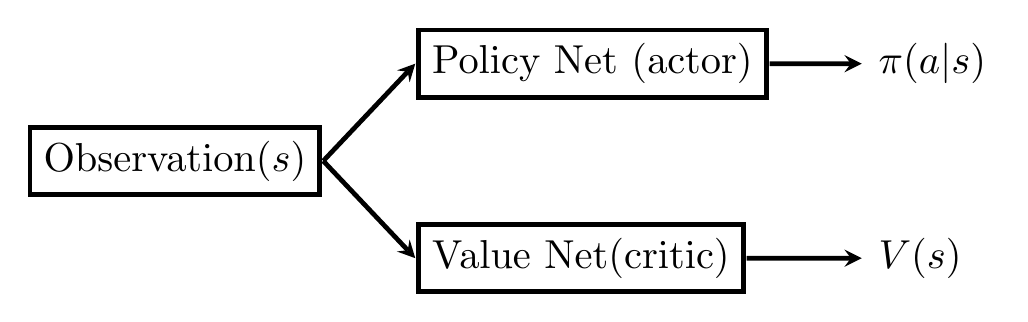
\begin{tikzpicture}[thick,scale=1.46, every node/.style={transform shape}, line width=0.6mm]
		\node[rectangle, draw] (obs) {Observation($s$)};
		\node[rectangle, draw, above right=2mm and 8mm of obs] (policy) {Policy Net (actor)};
		\node[rectangle, draw, below right=2mm and 8mm of obs] (value) {Value Net(critic)};
		\node[right=8mm of policy] (pi) {$\pi(a|s)$};
		\node[right=10mm of value] (v) {$V(s)$};
		\draw[-stealth] (obs.east) -- (policy.west);
		\draw[-stealth] (obs.east) -- (value.west);
		\draw[-stealth] (policy.east) -- (pi.west);
		\draw[-stealth] (value.east) -- (v.west);
	\end{tikzpicture}
	\caption[a2cflow]{Schematic on actor-critic architeture}
	\label{fig:a2cflow}
\end{figure}
The problems of this algorithm is the fact that is on-policy and sensible to hyperparameters, in order to improve performance, stability and efficiency the \acrshort{sac} was created.
\acrshort{sac} is able to do it introducing multiple components such as : 
\begin{itemize}
	\item a large buffer memory is needed to efficiently update the weights using previous history increasing in this way stability and switching to an off-policy method instead of an on-policy one.
	\item A target network of the critic net is introduced to improve the stability and efficiency of learning to approximate the value state, differently from the \acrshort{dqn} updating target network will follow the procedure of \textbf{soft functions update}. Shortly, this means that the values will use a factor to combine new and old weights obtained from the update step, to do this a loss value of state ($J_{V}$) and action ($J_{Q}$) function must be defined.
	\begin{equation}\label{state of calue loss}
		J_{V}(\psi)= \mathbb{E}_{s \sim S}\left[ \frac{1}{2} (V_\psi(s_t) - \mathbb{E}_{a_t \sim \pi_\phi}[Q_\theta(s_t,a_t) - \log \pi_{\phi}(a_t|s_t)])^2 \right]
	\end{equation}
	\begin{equation}\label{state of action loss}
		J_{Q}(\theta)= \mathbb{E}_{s \sim S, a \sim A }\left[\frac{1}{2}(Q_\theta(s_t,a_t) - r(s_t,a_t) + \gamma \mathbb{E}_{s_{t+1} \sim p}[V_{\overline{\psi}}(s_{t+1})] )^2 \right]
	\end{equation}
	\item the maximum entropy of reinforcement learning is introduced to increase the exploration of environment, improve learning and reduce sensibility to hyperparameters.The loss of this maximum entropy was transformed for this case from the "classical" one considering the use of a neural network and introducing an input noise vector($\epsilon_t$) sampled from the a fixed spherical gaussian distribution to calculate the action.\\
	Output action of neural network and input noise from currrent state can be expressed as follows $a_t = f_\phi(\epsilon_t;s_t)$ bringing to the loss formula:
	\begin{equation}\label{policy loss}
		J_{\pi}(\phi)= \mathbb{E}_{s \sim S, \epsilon_t \sim \mathcal{N}}\left[ \log \pi_{\phi}(f_\phi(\epsilon_t;s_t)) - Q_{\theta}(s_t, f_\phi(\epsilon_t;s_t))\right]
	\end{equation}
\end{itemize}
For more details on how these formulas have been obtained and experimental results refer to the original paper \cite{DBLP:journals/corr/abs-1801-01290}, to avoid confusion the pseudocode will be showed later considering that there are variations from the original implementation to create a quantum version, so that later it would be possible to confront classical and quantum algorithm.
\subsection{Quantum computing}
Quantum computing is a field that originated around the 1980s by numerous physicists, Paul Benioff was first to introduce the idea of a Turing machine that used quantum mechanics to make calculation. Richard Feynman and Yuri Manin suggested to use it for efficient simulation on quantum mechanics systems. Futhermore David Deutsch asked if using physical laws it was possible to derive a stronger version of the Church-Turing thesis introducing the concept of Universal Quantum Computing, this conjecture isn't still demonstrated but has paved the way for current concept. In order to introduce quantum computing it is necessary to understand what is a quantum bit, circuit and logic gate, keeping in mind that even if the following representation is an abstraction there is a physical implementation for all this components.
\subsubsection{Quantum bits}
Quantum bits or qubits are the analogous of classical bits which are used as a fundamental concept for computation and information forming a computational bases states. As the bits can have two possible states 0 and 1, the qubits, thanks to the discretized energy on a microscopic level, can have a quantum state $\ket{0}$ and $\ket{1}$. Differently from their classical counterparts and thanks to the quantum mechanics, the qubits can be in a possible \textit{linear combination} even known as \textit{superposition} of states:
\begin{equation}\label{superposition}
	\ket{\psi} = \alpha \ket{0} + \beta \ket{1}
\end{equation}
The numbers $\alpha$ and $\beta$ are complex even known as \textit{amplitudes}, so a qubit can be represented as a two-dimensional complex vector space. A fundamental condition is applied on these numbers to respect the statistical view of quantum mechanics, when a qubit is measured a probability of being on the quantum state is associated. These probabilities can be represented as $|\alpha|^2$ to be in state $\ket{0}$ and $|\beta|^2$ in state $\ket{1}$, for natural statistic normalization these number must have the condition $|\alpha|^2 + |\beta|^2 = 1$.Geometrically this can be interpreted as the fact that qubit states must be normalized in order to have length 1 and be rewritten using real numbers as:
\begin{equation}
	\ket{\psi} = e^{i\gamma} \bigg( \cos{\frac{\theta}{2}} \ket{0} + e^{i\varphi} \sin{\frac{\theta}{2}} \ket{1}\bigg)
\end{equation}
with $\gamma, \theta, \varphi \in R$. Due to the fact that there are no observables effects with a global phase, it is possible to ignore $e^{i\gamma}$ giving the reduced formula:
\begin{equation}\label{angle qubits}
	\ket{\psi} = \cos{\frac{\theta}{2}} \ket{0} + e^{i\varphi} \sin{\frac{\theta}{2}} \ket{1}
\end{equation}
This allows to introduce a three-dimensional sphere representation called \textbf{Bloch sphere} showed in figure \ref{bloch sphere}, which allows to represented any possible superposition of states in a qubit.
\begin{figure}[!ht]
	\centering
	\scalebox{1.8}{
	\begin{tikzpicture}[line cap=round, line join=round, >=Triangle]
		\clip(-2.19,-2.49) rectangle (2.66,2.58);
		\draw [shift={(0,0)}, lightgray, fill, fill opacity=0.1] (0,0) -- (56.7:0.4) arc (56.7:90.:0.4) -- cycle;
		\draw [shift={(0,0)}, lightgray, fill, fill opacity=0.1] (0,0) -- (-135.7:0.4) arc (-135.7:-33.2:0.4) -- cycle;
		\draw(0,0) circle (2cm);
		\draw [rotate around={0.:(0.,0.)},dash pattern=on 3pt off 3pt] (0,0) ellipse (2cm and 0.9cm);
		\draw (0,0)-- (0.70,1.10);
		\draw [->] (0,0) -- (0,2);
		\draw [->] (0,0) -- (-0.81,-0.79);
		\draw [->] (0,0) -- (2,0);
		\draw [dotted] (0.7,1)-- (0.7,-0.46);
		\draw [dotted] (0,0)-- (0.7,-0.46);
		\draw (-0.08,-0.3) node[anchor=north west] {$\varphi$};
		\draw (0.01,0.9) node[anchor=north west] {$\theta$};
		\draw (-1.10,-0.72) node[anchor=north west] {$\mathbf {\hat{x}}$};
		\draw (2.07,0.3) node[anchor=north west] {$\mathbf {\hat{y}}$};
		\draw (-0.5,2.6) node[anchor=north west] {$\mathbf {\hat{z}=|0\rangle}$};
		\draw (-0.4,-2) node[anchor=north west] {$-\mathbf {\hat{z}=|1\rangle}$};
		\draw (0.4,1.65) node[anchor=north west] {$\ket{\psi}$};
		\scriptsize
		\draw [fill] (0,0) circle (1.5pt);
		\draw [fill] (0.7,1.1) circle (0.5pt);
	\end{tikzpicture}
	}
	\caption[The bloch sphere]{Representation of a qubit the Bloch sphere}
	\label{bloch sphere}
\end{figure}

This formalism can be extended  for the case of multiple qubits, if for example a system is composed of two separable qubits $\ket{\psi}$ and $\ket{\phi}$ then it is possible to construct their representation $\ket{\nu}$ using the dot product as follows:
\begin{align*}
	\ket{\psi} &= \alpha \ket{0} + \beta \ket{1} \qquad
	\ket{\phi} = \gamma \ket{0} + \delta \ket{1}\\
	\ket{\nu} &= \ket{\psi} \otimes \ket{\phi} = \alpha\gamma \ket{00} + \alpha\delta \ket{01} + \beta\gamma \ket{10} + \beta\delta\ket{11}\\
\end{align*}
The previous form of $\ket{00}$ is only an abbreviation for the form $\ket{0} \otimes \ket{0}$,
normalization must be still valid so the sum of all amplitudes squared must give 1, in other words $|\alpha\gamma|^2  + |\alpha\delta|^2  + |\beta\gamma|^2  + |\beta\delta|^2 = 1$ if that is not the case it is possible to normalize it dividing by the root square of the squared sum. As it can be seen with only two qubits there are four quantum states, if for example we had $N$ qubits then there would be $2^N$ possible states giving a tremendous advantage on the information that can be stored instead of the classical approach.
Furthermore thanks to the fact that this is a multi dimensional space a matrix representation to give the following formalism:
\begin{align*}
	\ket{0} =   
		\begin{bmatrix}
			1 \\
			0
		\end{bmatrix}
	\qquad
	\ket{1} &=
	   \begin{bmatrix}
	   	0 \\
	   	1
	   \end{bmatrix}
    \qquad
    \ket{\psi} =
   		\begin{bmatrix}
   		 \alpha \\
   		 \beta
   		\end{bmatrix}
   	\qquad
   	\ket{\phi} =
   		\begin{bmatrix}
   		\gamma \\
   		\delta
   		\end{bmatrix}\\
   		\ket{\nu} &= \ket{\psi} \otimes \ket{\phi} = 
   		\begin{bmatrix}
   			\alpha\gamma & \alpha\delta\\
   			\beta\gamma  & \beta\delta
   		\end{bmatrix}\\
\end{align*}
In case a measurement is applied on subsets of qubits, for example on the first qubit measuring if the state is $\ket{0}$ then the post-measurement state will be:
\begin{equation}\label{post measurement}
		\ket{\nu'} = \frac{\alpha\gamma\ket{00} + \alpha\delta \ket{01}}{\sqrt{|\alpha\gamma|^2 + |\alpha\delta|^2}}
\end{equation}
the denominator is due to normalization after measurement in order to respect the condition that squared amplitudes summed is 1.\\
Quantum mechanics allows even some particular states called \textit{Bell states or EPR pair} which are not separable such as this one:
\begin{equation}\label{bell state}
	\frac{\ket{00} + \ket{11}}{\sqrt{2}}
\end{equation}
even if it seems to be completely normal, notice that in case a measurement is applied on any of the two qubits it is possible to know immediately with certainity what state is in the other one. So there is a \textit{correlation} between the qubits, point is that this type of correlation is \textbf{stronger than any kind that could exist classicaly}. This correlation is known as \textbf{entanglement}, is at the basis of many quantum algorithms and has been proven to be valid even on distance of galaxies. This doesn't violate Einstein general relativity because the information even if using this quantum property in any case can't exceed the speed of light. Now that the separated and entangled states have been introduced it is time to see how the qubits can be manipulated using the \textbf{gates and circuits}.
\subsubsection{Quantum gates and circuits}
As classical computation uses \textit{wires} amd \textit{logic gates}, quantum computing does the same. Main difference is that for example quantum gates such as the equivalent quantistic NOT act linearly instead of non-linearly, the reason is due to the fact that if non-linearity was allowed then empirically there would be paradoxes, such as violations of the second law of thermodynamics, faster than light communications and time travels. Taking advantage of the linear proprierty it is possible to give a matrix form of such as NOT, in fact a NOT gate classicaly invert 0 to 1, what happens on quantum computing is:
\begin{equation*}
	\alpha \ket{0} + \beta \ket{1} \to \beta \ket{0} + \alpha \ket{1}
\end{equation*}
in matrix form it can be translated as:
\begin{equation*}
	X = \begin{bmatrix}
		0 & 1 \\
		1 & 0
	\end{bmatrix}
	\to
	X \begin{bmatrix}
		\alpha \\
		\beta
	\end{bmatrix}
	= \begin{bmatrix}
		\beta \\
		\alpha
	\end{bmatrix}
\end{equation*}
In addition to the linearity of quantum gates, it is necessary to remember that these operations must respect the condition of normalization equal to 1. This can be translated to the condition that any matrix $U$ representing a quantum gate, must be unitary. This can be formalized using the \textit{adjoint} of $U^\dag$, which means complex conjugating and transposing the elements of U, as the condition $U^\dag U = 1$. This can be even interpreted as the fact that any kind of quantum operation applied is reversible, so by applying another one is possible to return at the initial state, which quantistically is the adjoint of operation applied.
The most used single qubit gates are the following:
\begin{equation*}
	X = \begin{bmatrix}
		0 & 1 \\
		1 & 0 
	\end{bmatrix}\qquad
	Y = \begin{bmatrix}
		0 & -i \\
		i & 0
	\end{bmatrix}\qquad
	Z = \begin{bmatrix}
		1 & 0 \\
		0 & -1 
	\end{bmatrix}
	H = \frac{1}{\sqrt{2}}\begin{bmatrix}
		1 & 1 \\
		1 & -1
	\end{bmatrix}
\end{equation*}
there are other gatex such as S, T and I, for the thesis they will not be necessary, but if interested feel free to check the book(put reference Nielsen Chang).The interesting part is that any kind of single qubit gate can be obtained from the generic form:
\begin{equation}\label{generic gate}
	U(\theta,  \phi, \lambda) =  \begin{bmatrix}
		\cos(\frac{\theta}{2}) & -e^{i\lambda} \sin(\frac{\theta}{2})\\
		e^{i\phi}\sin(\frac{\theta}{2}) & e^{i(\phi+ \lambda)}\cos(\frac{\theta}{2})
	\end{bmatrix}
\end{equation}
for confirmation as an example notice that $H = U(\frac{\pi}{2}, 0, \pi)$.\\
Now as there a single qubit gates, it is possible to extend the concept introducing \textbf{multiple qubit gates}. These, differently from the single qubits using multiple of them, for example one that will be used extensively is the \textit{controlled-NOT} or CNOT gate which has the following form:\\
\begin{center}
	\begin{quantikz}[scale = 3.0]
		 &  \ctrl{1} & \qw\\
		 &  \targ{}  & \qw
	\end{quantikz}
\end{center}
\begin{equation*}
	CNOT = 
	\begin{bmatrix}
		1 & 0 & 0 & 0 \\
		0 & 1 & 0 & 0 \\
		0 & 0 & 0 & 1 \\
		0 & 0 & 1 & 0
	\end{bmatrix}
\end{equation*} 
This gate function by using a control qubit which is the black dot and only if the control qubit is $\ket{1}$ applies to the target qubit $\oplus$ which is the addition modulo two operation that on a two basis computational state means to flip it. The horizontal line repreent the wire used to transfer the qubit. Formally CNOT is defined as:
\begin{equation*}
	\ket{00} \to \ket{00} \qquad \ket{01} \to \ket{01} \qquad \ket{10} \to \ket{11} \qquad \ket{11} \to \ket{10}
\end{equation*}
The import point is that this circuit is like it applies an $X$ gate, in fact it is possible to subsitute with other single qubit gate. There are other multi qubit gates such as \textit{toffoli}, \textit{swap} and many others, but they will not be used in this thesis.
The reason for which \textbf{CNOT is largely used because it can introduce the entanglement effect on qubits}, this is particularly important to efficiently explot the quantum advantage. For example the \ref{bell state} can be obtained with the following circuit:
\begin{center}
	\begin{quantikz}[scale = 3.0]
		\lstick{$\ket{0}$} & \gate{H} &  \ctrl{1} & \qw\\
		\lstick{$\ket{0}$} & \qw &  \targ{}  & \qw
	\end{quantikz}
\end{center}
Now that gates and wires have been introduced it is not necessary to introduce onle last component the measurement gate, in fact after the qubits are manipulated it is necessary to extract the information on these. In order to do that a measurement basis can be decided and quantum computing allows more than the classical basis of $\ket{0}$ and $\ket{1}$, but only this one will be used.As said the measurement consist of extracting information, but for the quantistic case this means distinguish the possible states, this is represented with the following symbol on circuits:
\begin{center}
	\begin{quantikz}[scale = 3.0]
		 & \meter{} & \qw
	\end{quantikz}
\end{center}
This measurement on the computational basis consist on using projectors of the possible eigenspaces, for the case of a generic qubit state projectors are $P_{0} = \ket{0} \bra{0}$ and $P_1 = \ket{1} \bra{1}$. The probability associated to be in one state, for example $\ket{0}$ can be defined as:
\begin{equation*}
	p(0) = tr(P_0 \ket{\psi}\bra{\psi}) = \bra{\psi}P_0\ket{\psi} = |\alpha_0|^2
\end{equation*}
The fully observable corresponding to a computational basis measurement is the Pauli-Z operator or the Z gate:
\begin{equation*}
	\sigma_z = \ket{0} \bra{0} - \ket{1}\bra{1} = Z
\end{equation*}
To work with quantum computing it is necessary to use statistics and in order to have the correct expectation value of $<\sigma_z>$ it is necessary to repeat multiple times the measurement to sample the possible values, his is usually represented as $S$ which is an abbreviation for \textit{shots}. In order to have the correct expectation with an error of at most $\epsilon$ conventional statistics can be used for example using the Bernoulli distribution.
Error gives a confidence interval $[p-\epsilon, p + \epsilon]$ which tells the proportion of samples that are in the interval. Statistically this can be associated to a $z$-value.
Estimating the error of a Bernoulli trial can be defined in different  ways, but the most preferred ways is by using the Wilson score interval \cite{10.2307/2276774}. Following that formula the overall error of estimation is bounded by the following equation:
\begin{equation*}
	\epsilon \le \sqrt{z^2 \frac{S +z^2}{4S^2}}
\end{equation*}
which can be inverted to calculate the S required:
\begin{equation*}
	S \le \frac{\epsilon^2 \sqrt{\frac{z^4(16\epsilon^2 + 1)}{\epsilon^4}} + z^2}{8\epsilon^2}
\end{equation*}
\subsubsection{Quantum decoherence}
There is phenomenon that needs to be considered when a quantum device is effectively used and that is \textbf{quantum decoherence}. The phenomenon is refeered to the effect of losing quantum coherence, this is obtained when the phase relation of the wave functions associated to different states is not valid anymore. This effects is mainly due to the fact that qubits are not completely isolated and interactions with environment introduce entanglement between them. The effect of quantum decoherence is problematic because implies loss of information stored.\\
This effect for quantum computing introduces non-linearity and is usually considered through quantities called \textit{decoherence times}. These are defined as $T_1$ and $T_2$, $T_1$ refers to \textit{relaxation time} which is the time taken to transition from $\ket{1} \to \ket{0}$. $T_2$ refers instead to \textit{dephasing time} that is the time for which qubits phase remains intact. These times are usually combined and used as costant decays for statistically say when quantum decoherence affect the qubits. Application of quantum gates influence the system by increasing the possibility of decoherence, for this reason \textbf{quantum error correction} has been developed. Problem is that these algorithms for error correction requires a lot of qubits and actually there are not physical devices with this capacity.\\
In order to deal with the quantum decoherence from environment and gates, new types of algorithms have been created with the requirement to use the least number of gates and operations required to successfully extract information.
\subsubsection{Encoding algorithms}
Working with quantum computers requires that information which needs to be analyzed and transformed needs to quantistic, there are different ways to encode: \textit{basis encoding, amplitude encoding, angle encoding.} There are even others in \cite{Schuld2021}, but these will be the ones used in this thesis.
Basis encoding is based on the fact that any bit is substituted with the qubit having corrisponding state value, for example $01001$ becomes $\ket{01001}$ using this strategy. As it is possible to notice this representation is not qubit efficent because it requires the same number of qubits for the associated bit of value, but the routine don't require many operations. Another strategy of encoding is called \textit{amplitude encoding}, which consist of taking the value of a classical vector $x$, normalize the values inside by normalizing the elements and associate to them an amplitude, like in this exxample:
\begin{align*}
	& x \to \sum_{k=1}^{2^n}|x_k| ^ 2 = 1 \\
	&x = \begin{bmatrix}
		x_1 \\
		\vdots \\
		x_{2^n}
	\end{bmatrix}
	 \leftrightarrow
	 \ket{x} = \sum_{j} x_j \ket{j}
\end{align*}
this kind of representation requrires very few qubits, but the routine required to encoded it is not applicable on the actual physical devices for their limited capabilities. The last strategy is the \textit{angle encoding} which consist on applying a rotation of the classical value along one axis, this is used because it can exhibit some similarities and proprierties to the amplitude encoding. It is not qubit efficient, but the routine can be applied using actual devices, formally it can be defines as follows:
\begin{equation*}
	x \to \ket{x} = \otimes_{i}^{n} R(x_i) \ket{0^i}
\end{equation*}
where $R$ can be $R_x, R_y, R_x$ so it is only necessary to apply one single rotation gate over every qubit using as angle the classical value.
%%
%%\subsection{Summary}
%%In this section it has been introduced reinforcement learning, deep reinforcement learning %%and quantum computing. It has been introduced the \acrlong{mdp} and Q-learning as basis for %%\acrlong{drl} and algorithms such as \acrlong{dqn} and \acrlong{sac} has been showed to deal %%with environments that can be discrete and continous. Futhermore it has been introduced %%quantum computing from the definition of qubits to gates and circuits. Quantum decoherence %%has been introduced such as one of the main limitations to the application of quantum %%algorithms using actual devices and encoding startegies has been explained on how to convert %%classical into quantum information. Now that introduction is finished, time has come to see %%how Quantum algorithms such as \acrfull{vqa} can be used to solve difficult environments and %%are applicable to actual \acrfull{qpu}.

\end{document}